% Original diagram of the completed study; no new algorithm or measurements.
\documentclass[tikz,border=3pt]{standalone}
\usepackage[T1]{fontenc}
\usepackage{lmodern}
\usetikzlibrary{arrows.meta,positioning,calc}
\definecolor{blue}{HTML}{0072B2}
\definecolor{orange}{HTML}{B36B00}
\definecolor{ink}{HTML}{303843}
\begin{document}
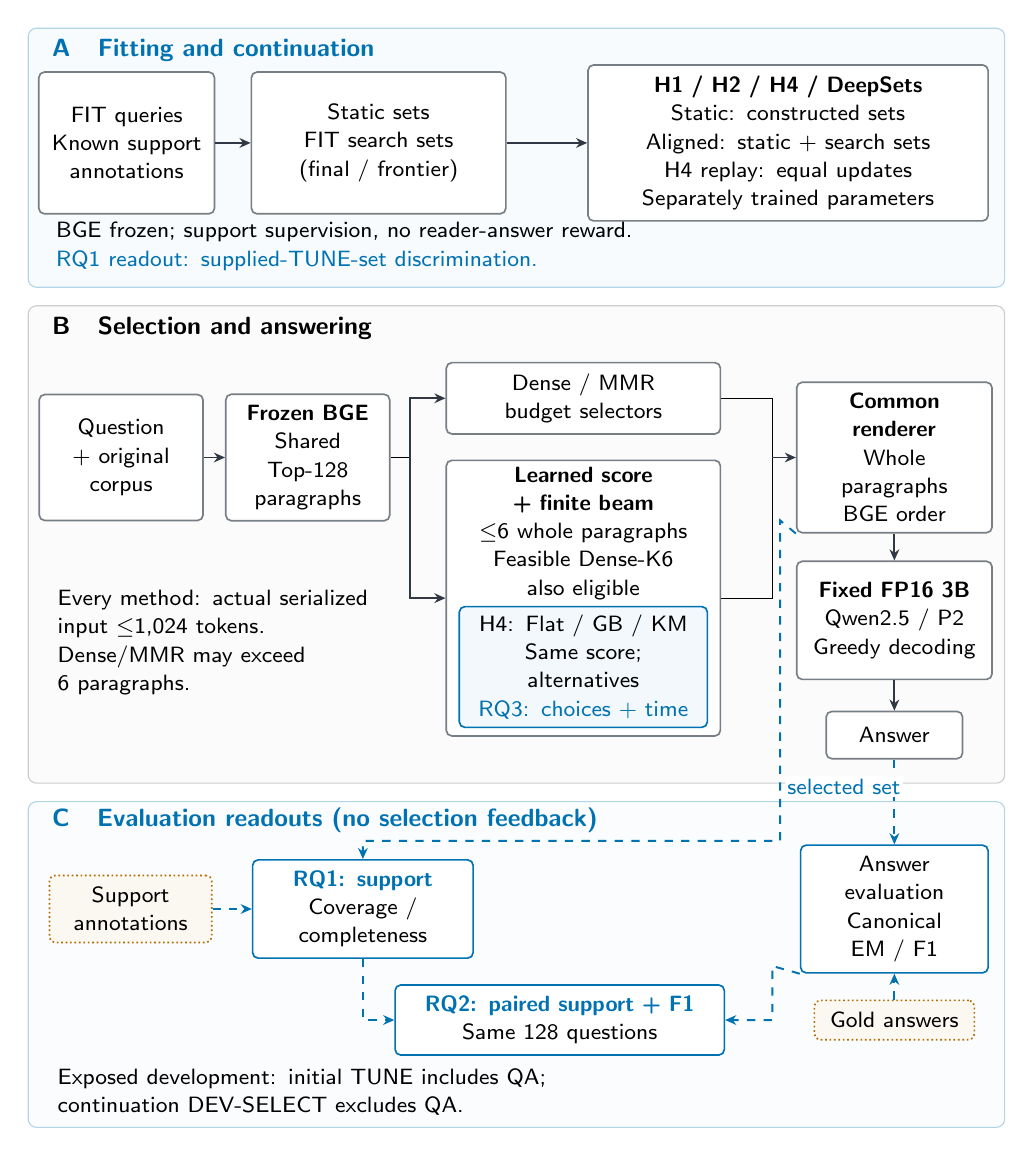
\begin{tikzpicture}[x=1cm,y=.94cm,
 font=\sffamily\fontsize{8.5}{10.2}\selectfont,
 box/.style={draw=ink!65,line width=.6pt,rounded corners=2pt,
    fill=white,align=center,inner sep=4pt},
 flow/.style={-{Stealth[length=4pt,width=3.5pt]},line width=.7pt,draw=ink},
 readout/.style={-{Stealth[length=4pt,width=3.5pt]},line width=.7pt,draw=blue,dashed},
 labeldata/.style={box,draw=orange,fill=orange!5,densely dotted},
 head/.style={anchor=west,font=\sffamily\bfseries\fontsize{9}{10.5}\selectfont}]

% A: fitting. Evaluation labels below are deliberately not connected to B inputs.
\filldraw[fill=blue!3,draw=blue!30,rounded corners=3pt] (0,11.4) rectangle (12.4,14.9);
\node[head,text=blue] at (.18,14.6) {A\quad Fitting and continuation};
\node[box,text width=1.95cm,minimum height=1.8cm] (fit) at (1.25,13.35)
 {FIT queries\\Known support\\annotations};
\node[box,text width=2.95cm,minimum height=1.8cm] (sets) at (4.45,13.35)
 {Static sets\\FIT search sets\\(final / frontier)};
\node[box,text width=4.8cm,minimum height=1.8cm] (models) at (9.65,13.35)
 {\textbf{H1 / H2 / H4 / DeepSets}\\Static: constructed sets\\Aligned: static + search sets\\H4 replay: equal updates\\Separately trained parameters};
\draw[flow] (fit)--(sets);
\draw[flow] (sets)--(models);
\node[align=left,anchor=west,text width=11.8cm] at (.23,11.95)
 {BGE frozen; support supervision, no reader-answer reward.\\
 \textcolor{blue}{RQ1 readout: supplied-TUNE-set discrimination.}};

% B: common candidate interface, parallel selectors, common rendering and reader.
\filldraw[fill=ink!2,draw=ink!25,rounded corners=3pt] (0,4.7) rectangle (12.4,11.15);
\node[head] at (.18,10.85) {B\quad Selection and answering};
\node[box,text width=1.8cm,minimum height=1.6cm] (inputs) at (1.18,9.1)
 {Question\\+ original\\corpus};
\node[box,text width=1.8cm,minimum height=1.6cm] (bge) at (3.55,9.1)
 {\textbf{Frozen BGE}\\Shared Top-128\\paragraphs};
\node[box,text width=3.2cm,minimum height=.8cm] (base) at (7.05,9.9)
 {Dense / MMR\\budget selectors};
\node[box,text width=3.2cm,minimum height=3.5cm] (learn) at (7.05,7.2) {};
\node[align=center,text width=3.15cm] at (7.05,8.08)
 {\textbf{Learned score}\\\textbf{+ finite beam}\\$\leq$6 whole paragraphs\\Feasible Dense-K6\\also eligible};
\node[box,fill=blue!5,draw=blue,text width=2.94cm,inner sep=3pt] at (7.05,6.27)
 {H4: Flat / GB / KM\\Same score; alternatives\\\textcolor{blue}{RQ3: choices + time}};
\node[box,text width=2.2cm,minimum height=1.5cm] (render) at (11.0,9.1)
 {\textbf{Common renderer}\\Whole\\paragraphs\\BGE order};
\node[box,text width=2.2cm,minimum height=1.5cm] (reader) at (11.0,6.9)
 {\textbf{Fixed FP16 3B}\\Qwen2.5 / P2\\Greedy decoding};
\node[box,text width=1.45cm,minimum height=.6cm] (answer) at (11.0,5.35) {Answer};
\draw[flow] (inputs)--(bge);
\coordinate (branch) at (4.85,9.1);
\draw (bge.east)--(branch);
\draw[flow] (branch)|-(base.west);
\draw[flow] (branch)|-(learn.west);
\coordinate (merge) at (9.45,9.1);
\draw (base.east)-|(merge);
\draw (learn.east)-|(merge);
\draw[flow] (merge)--(render.west);
\draw[flow] (render)--(reader);
\draw[flow] (reader)--(answer);
\node[align=left,anchor=west,text width=4.35cm] at (.25,6.6)
 {Every method: actual serialized\\input $\leq$1,024 tokens.\\Dense/MMR may exceed\\6 paragraphs.};

% C: one-way readouts; separate support and answer labels.
\filldraw[fill=blue!2,draw=blue!30,rounded corners=3pt] (0,.05) rectangle (12.4,4.45);
\node[head,text=blue] at (.18,4.2) {C\quad Evaluation readouts (no selection feedback)};
\node[labeldata,text width=1.78cm,minimum height=.85cm] (support) at (1.3,3.0)
 {Support\\annotations};
\node[box,draw=blue,text width=2.52cm,minimum height=1.1cm] (seval) at (4.25,3.0)
 {\textcolor{blue}{\textbf{RQ1: support}}\\Coverage /\\completeness};
\node[box,draw=blue,text width=3.9cm,minimum height=.85cm] (joint) at (6.75,1.5)
 {\textcolor{blue}{\textbf{RQ2: paired support + F1}}\\Same 128 questions};
\node[box,draw=blue,text width=2.1cm,minimum height=.95cm] (aeval) at (11.0,3.0)
 {Answer evaluation\\Canonical EM / F1};
\node[labeldata,text width=1.75cm,minimum height=.5cm] (gold) at (11.0,1.5) {Gold answers};
\draw[readout] (support)--(seval);
\draw[readout] (seval.south)|-(joint.west);
\draw[readout] (aeval.south west)--(9.45,2.23)|-(joint.east);
\draw[readout] (answer)--(aeval);
\draw[readout] (gold)--(aeval);
\draw[readout] (render.south west) -- (9.55,8.25) -- (9.55,3.92) -- (4.25,3.92) -- (seval.north);
\node[anchor=west,fill=white,text=blue,inner sep=1pt] at (9.6,4.65) {selected set};
\node[align=left,anchor=west,text width=11.8cm] at (.25,.52)
 {Exposed development: initial TUNE includes QA;\\
 continuation DEV-SELECT excludes QA.};
\end{tikzpicture}
\end{document}
